\documentclass{beamer}
\setbeamertemplate{caption}[numbered]
\usetheme[numbers, totalnumbers, compress, nologo]{Statmod}

\title[Синолитические сети в класс. мозговой активности]{Синолитические сети в классификации мозговой активности}

\author[Власенко Д.В.]{Власенко Даниил Владимирович, гр.19.Б04-мм}

\institute[Санкт-Петербургский Государственный Университет]{%
	\small
	Научный руководитель: к.ф.-м.н. Шпилёв П.В.\\ \vspace{0.5cm}
	Санкт-Петербургский государственный университет\\
	Прикладная математика и информатика\\
	Вычислительная стохастика и статистические модели\\
	\vspace{1.25cm}
	Отчет по научно-исследовательской работе}

\date[Зачет]{Санкт-Петербург, 2023}

\makeatletter
\newcommand*{\rom}[1]{\expandafter\@slowromancap\romannumeral #1@}
\newcommand\setItemnumber[1]{\setcounter{enum\romannumeral\@enumdepth}{\numexpr#1-1\relax}}
\makeatother

\usepackage{amsmath,amssymb,amsthm,amscd,amsfonts, mathtools}
\usepackage[utf8]{inputenc}
\usepackage[english, russian]{babel}
\usepackage{wrapfig}
\usepackage{multirow}

\newtheorem{definition_}{Определение}
\newtheorem{target_}{Цель работы}
\newtheorem{prob_task}{Вероятностная постановка задачи классификации}
\newtheorem{algo_task}{Алгоритмическая постановка задачи классификации}
\newtheorem{prob_def}{Вероятностное определение $w_{ij}^k$}
\newtheorem{algo_def}{Алгоритмическое определение $w_{ij}^k$}

\begin{document}
	\title[Синолитические сети в класс. мозговой активности]{Синолитические сети в классификации мозговой активности}
	
	\author[Власенко Д.В.]{Власенко Даниил Владимирович, гр.19.Б04-мм}
	
	\institute[Санкт-Петербургский Государственный Университет]{%
		\small
		Научный руководитель: к.ф.-м.н. Шпилёв П.В.\\ \vspace{0.5cm}
		Санкт-Петербургский государственный университет\\
		Прикладная математика и информатика\\
		Вычислительная стохастика и статистические модели\\
		\vspace{1.25cm}
		Отчет по научно-исследовательской работе}
	
	\date[Зачет]{Санкт-Петербург, 2023}
	
		
	\begin{frame}
		\titlepage
	\end{frame}

	\section{Введение}
	\subsection{фМРТ}
	\begin{frame}		
		\begin{definition_}
			Функциональная магнитно-резонансная томография или фМРТ~--- разновидность магнитно-резонансной томографии, которая проводится с целью измерения изменений в токе крови, вызванных нейронной активностью головного мозга. 
		\end{definition_}
		
		\begin{figure}
			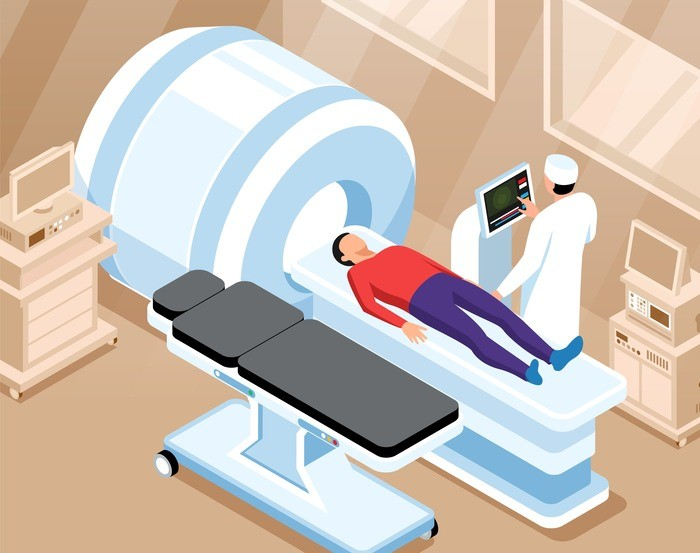
\includegraphics[width=5cm]{../images/fmri_1.jpeg}
			\caption{фМРТ сканер.} 
			\label{fg:1}
		\end{figure}	
	\end{frame}





\end{document}